\section{Application overview}
For us to create a system that can implement the fingerprinting technique in a suitable way, we decided to develop a mobile application. 
The benefit of using a mobile application rests on the fact that typical mobile devices already have the capability to interact and collect data from Bluetooth devices, such as Bluetooth beacons. 
This allowed us to integrate the process of collecting the data, doing classification, and applying the resulting classification model to conduct experiments within the same system.

A primary function of the application is to collect data from the aforementioned beacons. 
As illustrated in figure \ref{fig:ScanAdvertisement}, when the device is running, it will scan for advertisement packets projected by the Bluetooth beacons.

\begin{figure}[H]
    \centering
    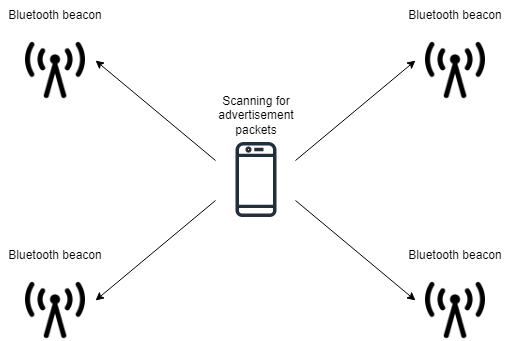
\includegraphics[width=0.5\textwidth]{images/ScanningForAdvertisement.drawio.png}
    \caption{}
    \label{fig:ScanAdvertisement}
\end{figure}

Each beacon advertises information, such as an identifier for the specific beacon and RSSI data. 
As described in section \ref{sec:fingerprinting}, fingerprinting consists of two phases. 
The first phase, where a map is generated based on the received Bluetooth signal, and a second phase, where the position of an unknown Bluetooth receiver is inferred. 
By using the advertisement packets projected by the beacons, the application is able to support the first phase of fingerprinting by generating a map of a room, through the collection of this advertisement data. 
The process of generating a map is illustrated in figure \ref{fig:CreateMap}, where a device running the application, and collecting the data, will be carried in a pattern around the room. 
Additionally, the beacons are positioned such that they outline the area of the room, as the ability to determine this area will be important during the second phase.

\begin{figure}[H]
    \centering
    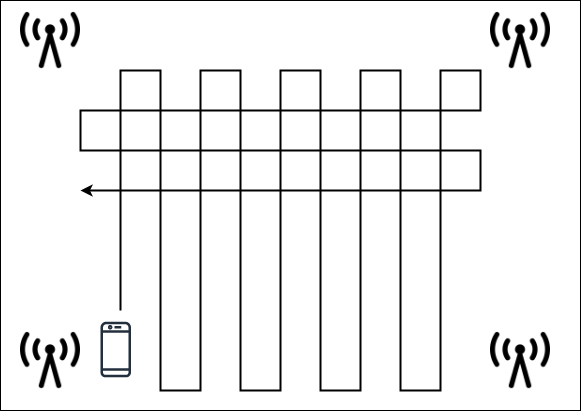
\includegraphics[width=0.5\textwidth]{images/CreateMap.drawio.png}
    \caption{}
    \label{fig:CreateMap}
\end{figure}

To support the second phase of fingerprinting, we have developed a classification module as part of the application. 
By collecting new data and using the map generated during the first phase, the classification module is trained to classify the position of other devices relative to the room. 
Using the trained model, the application is able to infer, with some certainty, that a device is either inside the room or outside the room.

